\subsubsection{Complex Ginzburg--Landau}
\label{sec:appendix_verification_gl}
\begin{figure}
    \centering
    \begin{minipage}[t]{0.48\textwidth}
        \centering
        \vspace{0pt}
        % This file was created by matlab2tikz.
%
\definecolor{mycolor1}{rgb}{0.20000,0.40000,0.60000}%
%
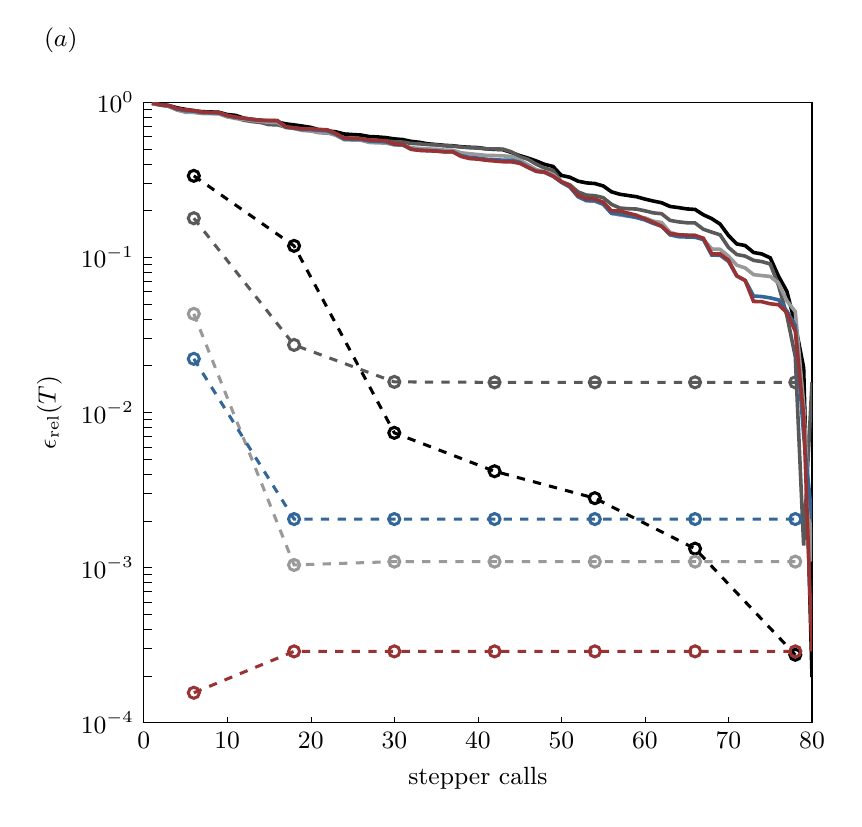
\begin{tikzpicture}

\begin{axis}[%
width=11.252in,
height=7.131in,
at={(1.887in,0.962in)},
scale only axis,
clip=true,
separate axis lines,
every outer x axis line/.append style={black},
every x tick label/.append style={font=\color{black}},
every x tick/.append style={black},
xmin=0,
xmax=80,
xlabel={stepper calls},
every outer y axis line/.append style={black},
every y tick label/.append style={font=\color{black}},
every y tick/.append style={black},
ymode=log,
ymin=0.0001,
ymax=1,
yminorticks=true,
ylabel={$\epsilon_{\mathrm{rel}}(T)$},
axis background/.style={fill=white},
clip=true,
clip mode=individual,
axis lines=box,
xtick pos=bottom,
ytick pos=left,
tick align=inside,
major tick length=2pt,
width=0.7\linewidth,
height=0.65\linewidth,
every axis/.append style={font=\fontsize{9}{9}\selectfont},xlabel style={font=\fontsize{9}{9}\selectfont},title style={font=\fontsize{9}{9}\selectfont},
legend style={font=\fontsize{8}{9}\selectfont,inner sep=1pt,row sep=1pt,column sep=2pt,nodes={scale=1.00},draw=none},legend image post style={xscale=0.35},
legend columns=1,
scaled x ticks=false,
tick label style={/pgf/number format/fixed,/pgf/number format/precision=2},
every x tick label/.append style={font=\fontsize{9}{9}\selectfont\color{black}},
every y tick label/.append style={font=\fontsize{9}{9}\selectfont\color{black}},
,,
colormap={sigmamap}{rgb(0.0000)=(0.0200,0.1880,0.3800); rgb(0.1000)=(0.0743,0.3456,0.5616); rgb(0.2000)=(0.1918,0.4980,0.7060); rgb(0.3000)=(0.3890,0.6708,0.8226); rgb(0.4000)=(0.7552,0.8682,0.9228); rgb(0.5000)=(0.9690,0.9689,0.9689); rgb(0.6000)=(0.9425,0.8044,0.7614); rgb(0.7000)=(0.8767,0.4910,0.4020); rgb(0.8000)=(0.7869,0.2866,0.2470); rgb(0.9000)=(0.6186,0.1239,0.1568); rgb(1.0000)=(0.4040,0.0000,0.1220)}
]
\addplot [color=black, line width=1.3pt, forget plot]
  table[row sep=crcr]{%
1	0.985165464502917\\
2	0.971048359830997\\
3	0.951205179050231\\
4	0.919681047700775\\
5	0.899249412820878\\
6	0.880805994430103\\
7	0.868459742494046\\
8	0.865199492680536\\
9	0.861114197062287\\
10	0.832525113113597\\
11	0.822398689108786\\
12	0.788670148690936\\
13	0.775021625627415\\
14	0.764549352578276\\
15	0.747746973613479\\
16	0.745712139733251\\
17	0.724965063859842\\
18	0.713974519830427\\
19	0.701444244155202\\
20	0.688482774619424\\
21	0.663182110301451\\
22	0.65435357265626\\
23	0.64407505382054\\
24	0.624129625964055\\
25	0.618414678614345\\
26	0.614229876610716\\
27	0.600565092768903\\
28	0.597031889384245\\
29	0.591240547176463\\
30	0.579989136718529\\
31	0.574332747631998\\
32	0.558906071472685\\
33	0.551424866729417\\
34	0.539182540890269\\
35	0.533524060767838\\
36	0.52717094141623\\
37	0.523571656178599\\
38	0.516042372207813\\
39	0.512332268723539\\
40	0.509670785497178\\
41	0.500782949538627\\
42	0.496546792309842\\
43	0.494342949858862\\
44	0.474330601756383\\
45	0.45263687517021\\
46	0.436463402022355\\
47	0.41765607247181\\
48	0.397465607198713\\
49	0.385282284592009\\
50	0.337283356987566\\
51	0.328513798162926\\
52	0.309670329668666\\
53	0.301926775381416\\
54	0.299026111763803\\
55	0.288612391923131\\
56	0.264457019190453\\
57	0.254980536533236\\
58	0.250205782373461\\
59	0.245812576451499\\
60	0.237374855379344\\
61	0.230549355537883\\
62	0.224861889966195\\
63	0.212799059810108\\
64	0.209293996703853\\
65	0.205196913687323\\
66	0.203571124582919\\
67	0.188035812467885\\
68	0.177630310730338\\
69	0.16372654312346\\
70	0.138302991694355\\
71	0.122002256923464\\
72	0.119097970006177\\
73	0.107519625210511\\
74	0.105067727551673\\
75	0.0992037278314537\\
76	0.0754210347718126\\
77	0.0602465034532608\\
78	0.0366705573794107\\
79	0.019419822005287\\
80	0.000197351436241734\\
};
\addplot [color=black, dashed, line width=1.1pt, mark size=2.0pt, mark=o, mark options={solid, black}, forget plot]
  table[row sep=crcr]{%
6	0.335159987761167\\
18	0.118531569790602\\
30	0.00739365023044105\\
42	0.00417927746508909\\
54	0.00280275867247948\\
66	0.001325154662104\\
78	0.000274288373235347\\
};
\addplot [color=white!35!black, line width=1.3pt, forget plot]
  table[row sep=crcr]{%
1	0.978599504948092\\
2	0.958939501992847\\
3	0.939693066967005\\
4	0.89261026284617\\
5	0.867840917394025\\
6	0.861406077656702\\
7	0.852698239057536\\
8	0.85017245615521\\
9	0.847032144185355\\
10	0.80729432471463\\
11	0.793416282120727\\
12	0.765630153360495\\
13	0.74988185038214\\
14	0.740470036675323\\
15	0.716426184465566\\
16	0.715341748661657\\
17	0.691584384991789\\
18	0.683455781101978\\
19	0.670675562334103\\
20	0.654454550999417\\
21	0.637112149433065\\
22	0.633257778866529\\
23	0.620317618750451\\
24	0.588720020973351\\
25	0.585945706960771\\
26	0.582267838430227\\
27	0.56742924037083\\
28	0.565364720145365\\
29	0.562807616623031\\
30	0.555634500442104\\
31	0.553314809191816\\
32	0.54238243410962\\
33	0.539039247828093\\
34	0.532643096219939\\
35	0.530584870874834\\
36	0.522539364472817\\
37	0.521445234589325\\
38	0.513154688684804\\
39	0.508839959353012\\
40	0.505939514085901\\
41	0.500655814429845\\
42	0.499712265513766\\
43	0.498404391560835\\
44	0.478878943258887\\
45	0.445626597424573\\
46	0.428464859611121\\
47	0.398258275036155\\
48	0.376128564976229\\
49	0.362789243735769\\
50	0.307295386037411\\
51	0.293601467871381\\
52	0.263957921658544\\
53	0.251759619862065\\
54	0.249676687234887\\
55	0.242489853789401\\
56	0.219495168292962\\
57	0.207859611903422\\
58	0.205754176866974\\
59	0.204741582868334\\
60	0.199458164115086\\
61	0.193520310988052\\
62	0.190931637714247\\
63	0.173087985360088\\
64	0.169340146062514\\
65	0.167072941945809\\
66	0.166542467767846\\
67	0.151614680982998\\
68	0.145368741746296\\
69	0.139618579434393\\
70	0.115866788291259\\
71	0.104232963892324\\
72	0.101843105302551\\
73	0.0955708834689444\\
74	0.0938174024887371\\
75	0.0906079543094753\\
76	0.0657956360552881\\
77	0.0418853536153708\\
78	0.0228826914806503\\
79	0.00138771895001788\\
80	0.0156460030015282\\
};
\addplot [color=white!35!black, dashed, line width=1.1pt, mark size=2.0pt, mark=o, mark options={solid, white!35!black}, forget plot]
  table[row sep=crcr]{%
6	0.178634994647454\\
18	0.0272494655305371\\
30	0.0157452937165598\\
42	0.0156391308471297\\
54	0.0156432097817025\\
66	0.0156460997728516\\
78	0.0156460065903751\\
};
\addplot [color=white!60!black, line width=1.3pt, forget plot]
  table[row sep=crcr]{%
1	0.983939814725101\\
2	0.958621292050389\\
3	0.941410908329715\\
4	0.890755899497388\\
5	0.861457015736498\\
6	0.859985130675222\\
7	0.845697130140114\\
8	0.84384524991711\\
9	0.840712634135543\\
10	0.806066660950854\\
11	0.785220616474763\\
12	0.776763649448303\\
13	0.761103340890232\\
14	0.75261633371115\\
15	0.740564558251317\\
16	0.739651588083636\\
17	0.686174570596409\\
18	0.676538220042228\\
19	0.65747615287434\\
20	0.651761925296852\\
21	0.640299018596555\\
22	0.636199216480547\\
23	0.610879445340382\\
24	0.573000938865489\\
25	0.570269997442903\\
26	0.568735320710756\\
27	0.550363133482551\\
28	0.546783209951033\\
29	0.545147664528803\\
30	0.530625903954825\\
31	0.528389559501782\\
32	0.508318851954079\\
33	0.503980652374716\\
34	0.499613192675354\\
35	0.49763637312336\\
36	0.490959101835251\\
37	0.490643493508232\\
38	0.472132561173985\\
39	0.46529930178891\\
40	0.459836536188394\\
41	0.454070526874192\\
42	0.453084808068927\\
43	0.450921515878575\\
44	0.446915469987828\\
45	0.423482412433708\\
46	0.395423667568545\\
47	0.367204866683023\\
48	0.356292784685205\\
49	0.341663964243568\\
50	0.306891857435353\\
51	0.285139234618715\\
52	0.246301072832208\\
53	0.231967547990899\\
54	0.230547619059275\\
55	0.221083463022862\\
56	0.192621792750176\\
57	0.187439295663882\\
58	0.184303648641886\\
59	0.182138524821364\\
60	0.179570703186825\\
61	0.171154224360516\\
62	0.167433487565166\\
63	0.145003386402656\\
64	0.139611153942317\\
65	0.139222997248754\\
66	0.138620251364076\\
67	0.130288551990365\\
68	0.113200339183079\\
69	0.112642085997531\\
70	0.101776616986649\\
71	0.0890035156036651\\
72	0.0854020580954648\\
73	0.077391766903902\\
74	0.0762840444580965\\
75	0.0753165799713176\\
76	0.0680914430609462\\
77	0.0523770125267109\\
78	0.0446863165468323\\
79	0.0113900519737571\\
80	0.00109306870352377\\
};
\addplot [color=white!60!black, dashed, line width=1.1pt, mark size=2.0pt, mark=o, mark options={solid, white!60!black}, forget plot]
  table[row sep=crcr]{%
6	0.0432217565843151\\
18	0.00104058419757173\\
30	0.00109300796967562\\
42	0.00109306851668768\\
54	0.00109306870455549\\
66	0.00109306870351742\\
78	0.00109306870352434\\
};
\addplot [color=mycolor1, line width=1.3pt, forget plot]
  table[row sep=crcr]{%
1	0.989811891709964\\
2	0.960431859012181\\
3	0.947709764979468\\
4	0.902376300114507\\
5	0.881075920619318\\
6	0.876674455805922\\
7	0.856885350128844\\
8	0.855090827494591\\
9	0.851761640525362\\
10	0.819320189184422\\
11	0.797292548273364\\
12	0.78806122225905\\
13	0.77276006590294\\
14	0.764282501804924\\
15	0.76071644434043\\
16	0.759703269063204\\
17	0.691619520587041\\
18	0.67967319361489\\
19	0.666621616328036\\
20	0.665504318632122\\
21	0.658670748743334\\
22	0.653705159150912\\
23	0.621556267060521\\
24	0.579768859923312\\
25	0.576997067249284\\
26	0.575868845616789\\
27	0.562810814189649\\
28	0.55797512494194\\
29	0.555658984500403\\
30	0.533488707883595\\
31	0.530480999056352\\
32	0.498123892171704\\
33	0.491116268851211\\
34	0.487948530398078\\
35	0.485573568159683\\
36	0.479551659861754\\
37	0.479359417296565\\
38	0.452077992888222\\
39	0.440933079350967\\
40	0.436152475342342\\
41	0.428890724024518\\
42	0.426217957695805\\
43	0.42258233338666\\
44	0.422254731169116\\
45	0.409952512737682\\
46	0.381810352992008\\
47	0.358308180091778\\
48	0.352175878101747\\
49	0.333306977167566\\
50	0.30424016970697\\
51	0.284178935698881\\
52	0.245756387656101\\
53	0.232000781397229\\
54	0.231310588412865\\
55	0.220004381709227\\
56	0.191907614754701\\
57	0.190463142463489\\
58	0.184969423564124\\
59	0.180402954768267\\
60	0.174144315703504\\
61	0.165465646833326\\
62	0.158712453070042\\
63	0.139617470060995\\
64	0.135879800133814\\
65	0.135207205933744\\
66	0.134716855584887\\
67	0.130151348694189\\
68	0.103306056164728\\
69	0.103176492744065\\
70	0.0941986632569092\\
71	0.0758320657443923\\
72	0.0710547597258276\\
73	0.0563570401697191\\
74	0.0558645644393192\\
75	0.0547663759366945\\
76	0.0531627847504146\\
77	0.0449587446280415\\
78	0.036338931906693\\
79	0.00714351915577783\\
80	0.002055929390514\\
};
\addplot [color=mycolor1, dashed, line width=1.1pt, mark size=2.0pt, mark=o, mark options={solid, mycolor1}, forget plot]
  table[row sep=crcr]{%
6	0.0221710184949555\\
18	0.00205572676526485\\
30	0.00205592952111303\\
42	0.00205592939052286\\
54	0.0020559293905168\\
66	0.00205592939051692\\
78	0.0020559293905112\\
};
\addplot [color=red!60!teal, line width=1.3pt, forget plot]
  table[row sep=crcr]{%
1	0.992325618839863\\
2	0.961016066817814\\
3	0.951208342921825\\
4	0.909270854860793\\
5	0.89254895682782\\
6	0.884815513639991\\
7	0.862290154659604\\
8	0.860415877005582\\
9	0.857853229850865\\
10	0.822332385875221\\
11	0.801433628859122\\
12	0.787904543949321\\
13	0.774317514752259\\
14	0.765141215814968\\
15	0.762530829118749\\
16	0.761325433853939\\
17	0.694682953325543\\
18	0.682341731535508\\
19	0.674346656399483\\
20	0.672786566648059\\
21	0.668200119625061\\
22	0.663293053353033\\
23	0.629081819149951\\
24	0.586888228823027\\
25	0.584317228262044\\
26	0.581314029745595\\
27	0.571490377868498\\
28	0.566770176814566\\
29	0.563935424311444\\
30	0.537455260735946\\
31	0.53422339882455\\
32	0.497334856023746\\
33	0.488809171678629\\
34	0.486072051456463\\
35	0.483504725005103\\
36	0.478304543183782\\
37	0.478240020525966\\
38	0.446736796169955\\
39	0.433120419580013\\
40	0.429548615138443\\
41	0.422298926512988\\
42	0.417698915367519\\
43	0.413275061006734\\
44	0.412531808256351\\
45	0.40388650613073\\
46	0.379494267012634\\
47	0.358844828047536\\
48	0.354638192262945\\
49	0.333453830121188\\
50	0.307032096596556\\
51	0.289435507933016\\
52	0.251135032099835\\
53	0.238193191630314\\
54	0.237783085631403\\
55	0.226677193556239\\
56	0.199360448424778\\
57	0.198959877325978\\
58	0.192612715272565\\
59	0.186689944541466\\
60	0.177117654749482\\
61	0.168016765002079\\
62	0.158442443672403\\
63	0.142320577140866\\
64	0.140036078567272\\
65	0.138761648579695\\
66	0.138314633879418\\
67	0.132805255890634\\
68	0.105232681267841\\
69	0.105081998102503\\
70	0.0959096699196229\\
71	0.0759144093102118\\
72	0.070894907510888\\
73	0.0519731430204992\\
74	0.0517514147346468\\
75	0.0501827934196301\\
76	0.049479744716153\\
77	0.0439304260189536\\
78	0.0333957003281456\\
79	0.00955117552443943\\
80	0.000288500251500087\\
};
\addplot [color=red!60!teal, dashed, line width=1.1pt, mark size=2.0pt, mark=o, mark options={solid, red!60!teal}, forget plot]
  table[row sep=crcr]{%
6	0.000156112389094138\\
18	0.000288490466867784\\
30	0.000288500251553511\\
42	0.00028850025150066\\
54	0.000288500251500851\\
66	0.000288500251497798\\
78	0.000288500251498943\\
};
\node[right, align=left, inner sep=0]
at (rel axis cs:-0.15,1.1) {$(a)$};
\end{axis}
\end{tikzpicture}%
    \end{minipage}
    \hfill
    \begin{minipage}[t]{0.48\textwidth}
        \centering
        \vspace{0pt}
        % This file was created by matlab2tikz.
%
\definecolor{mycolor1}{rgb}{0.20000,0.40000,0.60000}%
%
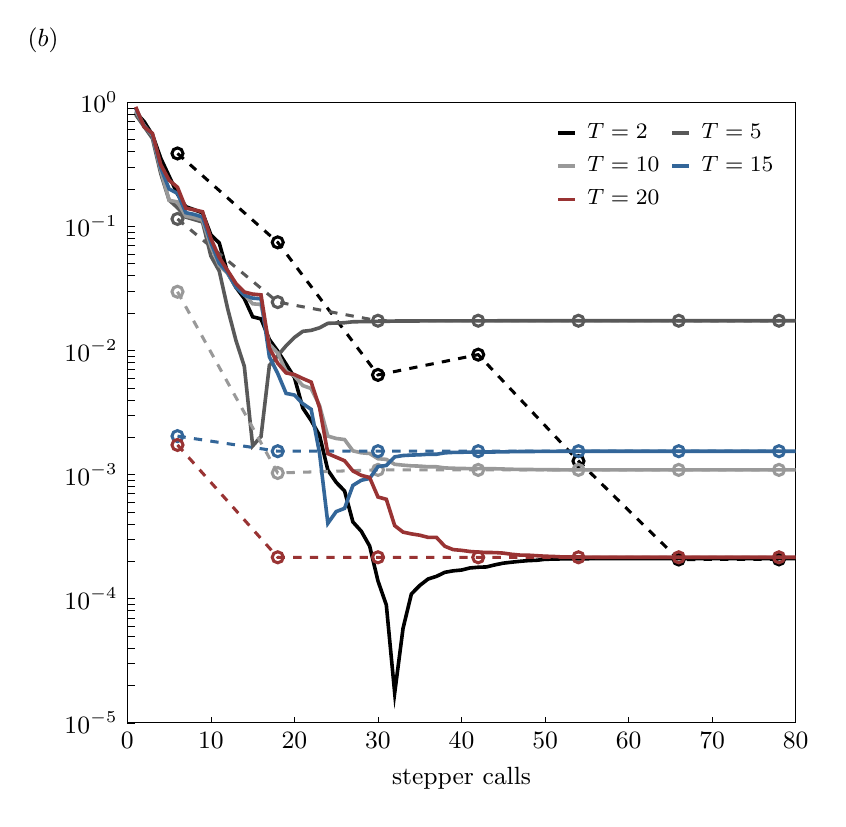
\begin{tikzpicture}

\begin{axis}[%
width=11.252in,
height=7.131in,
at={(1.887in,0.962in)},
scale only axis,
clip=true,
separate axis lines,
every outer x axis line/.append style={black},
every x tick label/.append style={font=\color{black}},
every x tick/.append style={black},
xmin=0,
xmax=80,
xlabel={stepper calls},
every outer y axis line/.append style={black},
every y tick label/.append style={font=\color{black}},
every y tick/.append style={black},
ymode=log,
ymin=1e-05,
ymax=1,
yminorticks=true,
axis background/.style={fill=white},
legend style={legend cell align=left, align=left},
clip=true,
clip mode=individual,
axis lines=box,
xtick pos=bottom,
ytick pos=left,
tick align=inside,
major tick length=2pt,
width=0.7\linewidth,
height=0.65\linewidth,
every axis/.append style={font=\fontsize{9}{9}\selectfont},xlabel style={font=\fontsize{9}{9}\selectfont},title style={font=\fontsize{9}{9}\selectfont},
legend style={font=\fontsize{8}{9}\selectfont,inner sep=1pt,row sep=1pt,column sep=2pt,nodes={scale=1.00},draw=none},legend image post style={xscale=0.35},
legend columns=2,
scaled x ticks=false,
tick label style={/pgf/number format/fixed,/pgf/number format/precision=2},
every x tick label/.append style={font=\fontsize{9}{9}\selectfont\color{black}},
every y tick label/.append style={font=\fontsize{9}{9}\selectfont\color{black}},
,,
colormap={sigmamap}{rgb(0.0000)=(0.0200,0.1880,0.3800); rgb(0.1000)=(0.0743,0.3456,0.5616); rgb(0.2000)=(0.1918,0.4980,0.7060); rgb(0.3000)=(0.3890,0.6708,0.8226); rgb(0.4000)=(0.7552,0.8682,0.9228); rgb(0.5000)=(0.9690,0.9689,0.9689); rgb(0.6000)=(0.9425,0.8044,0.7614); rgb(0.7000)=(0.8767,0.4910,0.4020); rgb(0.8000)=(0.7869,0.2866,0.2470); rgb(0.9000)=(0.6186,0.1239,0.1568); rgb(1.0000)=(0.4040,0.0000,0.1220)}
]
\addplot [color=black, line width=1.3pt]
  table[row sep=crcr]{%
1	0.832142165809318\\
2	0.698807622707636\\
3	0.546807535646839\\
4	0.353256308468127\\
5	0.2533545113672\\
6	0.181829801602638\\
7	0.143961931458514\\
8	0.136069474952372\\
9	0.128276084439533\\
10	0.0853515771514262\\
11	0.0733972032655607\\
12	0.0421167159491625\\
13	0.032179511831854\\
14	0.026197264594499\\
15	0.0186703519100572\\
16	0.0179558484860287\\
17	0.0122477491436808\\
18	0.00987930822292705\\
19	0.00776495043096266\\
20	0.00605286229772802\\
21	0.00343739612353565\\
22	0.00272330657881337\\
23	0.00207295030764483\\
24	0.00108590094293048\\
25	0.000864740726484522\\
26	0.000738121574372372\\
27	0.000414905706821819\\
28	0.00034958297313094\\
29	0.000265902270606906\\
30	0.00013885897151188\\
31	8.89550707338264e-05\\
32	1.73790854390435e-05\\
33	5.76632853457698e-05\\
34	0.000109156501001198\\
35	0.00012774614898567\\
36	0.000144046922404943\\
37	0.00015125888994871\\
38	0.000163039715967061\\
39	0.000167572474343433\\
40	0.000170111260942139\\
41	0.000176730335302363\\
42	0.000179193232154384\\
43	0.000180193469332686\\
44	0.000187283454047588\\
45	0.000193282521925197\\
46	0.000196773393056463\\
47	0.000199941632828961\\
48	0.00020259610362408\\
49	0.000203846130160141\\
50	0.000207689293072777\\
51	0.000208237218434015\\
52	0.000209155919455236\\
53	0.000209450502219311\\
54	0.000209536602094388\\
55	0.000209777778221061\\
56	0.000210214244888818\\
57	0.000210347836618805\\
58	0.000210400349410914\\
59	0.000210438042734826\\
60	0.000210494518788903\\
61	0.00021053015716279\\
62	0.000210553322293998\\
63	0.000210591647673277\\
64	0.000210600334145073\\
65	0.000210608254088011\\
66	0.000210610705413184\\
67	0.000210628975313441\\
68	0.000210638519721798\\
69	0.00021064846641863\\
70	0.000210662651566689\\
71	0.000210669744848924\\
72	0.000210670730477753\\
73	0.00021067379487986\\
74	0.00021067430095941\\
75	0.000210675244846075\\
76	0.000210678230149818\\
77	0.000210679715527429\\
78	0.000210681515133548\\
79	0.000210682541956614\\
80	0.000210683452492522\\
};
\addlegendentry{$T=2$}

\addplot [color=black, dashed, line width=1.1pt, mark size=2.0pt, mark=o, mark options={solid, black}, forget plot]
  table[row sep=crcr]{%
6	0.38634485377839\\
18	0.0742417278942887\\
30	0.00635197919233409\\
42	0.00924881520992697\\
54	0.00128367921167339\\
66	0.000206791538716321\\
78	0.000207192745182013\\
};
\addplot [color=white!35!black, line width=1.3pt]
  table[row sep=crcr]{%
1	0.794201241174241\\
2	0.636392197071579\\
3	0.511097089381333\\
4	0.265419020726859\\
5	0.162490441026057\\
6	0.141282246946287\\
7	0.118583735195212\\
8	0.113387263024999\\
9	0.108295982662846\\
10	0.0575898627114288\\
11	0.0436663052599052\\
12	0.0217657425047832\\
13	0.0120211522516976\\
14	0.0074518699460532\\
15	0.00170193007565686\\
16	0.00202554643688287\\
17	0.00758054743888711\\
18	0.00906925911452958\\
19	0.0109020267657692\\
20	0.0127229895482339\\
21	0.0142466131427801\\
22	0.014511566017313\\
23	0.0152074097413436\\
24	0.0165363359023962\\
25	0.0166275793436142\\
26	0.0167221533865549\\
27	0.017020440194329\\
28	0.017052879094671\\
29	0.0170842802529692\\
30	0.0171531143988702\\
31	0.0171705074859301\\
32	0.0172345496823139\\
33	0.0172498491050995\\
34	0.0172727133096399\\
35	0.0172784599704133\\
36	0.0172960038585485\\
37	0.0172978670507015\\
38	0.01730889148876\\
39	0.0173133715233898\\
40	0.0173157228794942\\
41	0.0173190670670061\\
42	0.0173195332858691\\
43	0.017320037760821\\
44	0.0173259167076527\\
45	0.0173337316030692\\
46	0.0173368796634658\\
47	0.0173412042420974\\
48	0.0173436768691506\\
49	0.0173448400265504\\
50	0.0173486162131316\\
51	0.0173493433608628\\
52	0.0173505716335023\\
53	0.017350966015995\\
54	0.0173510185610251\\
55	0.0173511600156901\\
56	0.0173515131306214\\
57	0.0173516525332058\\
58	0.0173516722123954\\
59	0.0173516795960179\\
60	0.0173517096502393\\
61	0.0173517359992392\\
62	0.017351744959992\\
63	0.0173517931405994\\
64	0.0173518010342846\\
65	0.0173518047589665\\
66	0.0173518054387212\\
67	0.0173518203585172\\
68	0.0173518252274636\\
69	0.0173518287235146\\
70	0.0173518399862865\\
71	0.0173518442887167\\
72	0.0173518449779994\\
73	0.0173518463888206\\
74	0.0173518466964082\\
75	0.0173518471354517\\
76	0.0173518497824039\\
77	0.0173518517715081\\
78	0.0173518530042554\\
79	0.0173518540916225\\
80	0.0173518547635486\\
};
\addlegendentry{$T=5$}

\addplot [color=white!35!black, dashed, line width=1.1pt, mark size=2.0pt, mark=o, mark options={solid, white!35!black}, forget plot]
  table[row sep=crcr]{%
6	0.114627266417663\\
18	0.0245110260665455\\
30	0.0173550749753947\\
42	0.0173553372422539\\
54	0.0173517356824942\\
66	0.017351859167501\\
78	0.0173518546728774\\
};
\addplot [color=white!60!black, line width=1.3pt]
  table[row sep=crcr]{%
1	0.84876248212394\\
2	0.649751643309823\\
3	0.540037042350577\\
4	0.281205903590061\\
5	0.161982206992004\\
6	0.157231809946868\\
7	0.120760737936852\\
8	0.117029821354168\\
9	0.112056444044837\\
10	0.0687652892723018\\
11	0.048285017579275\\
12	0.0417577423341335\\
13	0.0322687478482075\\
14	0.0282339730743595\\
15	0.0237409519465848\\
16	0.0234741596608912\\
17	0.0112296011081531\\
18	0.00950138804760071\\
19	0.00682450635838535\\
20	0.00619634569975223\\
21	0.00521017233758741\\
22	0.00493419836620897\\
23	0.00360091672537679\\
24	0.00204089843628622\\
25	0.00195294587640533\\
26	0.00191430181873946\\
27	0.00155264879828137\\
28	0.00149756666011107\\
29	0.00147789912083002\\
30	0.00134143911241692\\
31	0.00132501903343994\\
32	0.00120988481005397\\
33	0.00119044401344739\\
34	0.00117515581497276\\
35	0.00116975101375087\\
36	0.0011554929174147\\
37	0.00115496662479683\\
38	0.00113086248234519\\
39	0.00112391470680959\\
40	0.00111957803700095\\
41	0.00111600433861349\\
42	0.00111552739337057\\
43	0.00111471028631988\\
44	0.00111352913783512\\
45	0.0011081362684778\\
46	0.00110309615758645\\
47	0.00109914002544802\\
48	0.00109794609075457\\
49	0.00109669697086278\\
50	0.00109437995187906\\
51	0.00109324886331059\\
52	0.00109167301886039\\
53	0.00109121922217887\\
54	0.00109118414593429\\
55	0.00109100173467356\\
56	0.00109057373932463\\
57	0.00109051293803442\\
58	0.00109048423798858\\
59	0.00109046877807932\\
60	0.00109045447447922\\
61	0.00109041790193447\\
62	0.00109040528986774\\
63	0.0010903459823417\\
64	0.00109033486099181\\
65	0.00109033423654462\\
66	0.00109033348021297\\
67	0.00109032532582996\\
68	0.00109031228143468\\
69	0.0010903119490669\\
70	0.00109030690376152\\
71	0.00109030227805846\\
72	0.00109030126088857\\
73	0.0010902994965216\\
74	0.00109029930624357\\
75	0.00109029917664437\\
76	0.00109029842187397\\
77	0.00109029714172199\\
78	0.00109029665316491\\
79	0.00109029500376933\\
80	0.00109029460601764\\
};
\addlegendentry{$T=10$}

\addplot [color=white!60!black, dashed, line width=1.1pt, mark size=2.0pt, mark=o, mark options={solid, white!60!black}, forget plot]
  table[row sep=crcr]{%
6	0.0296986393320929\\
18	0.00102941666107282\\
30	0.00109027663329274\\
42	0.00109029472584195\\
54	0.00109029460615259\\
66	0.00109029460601256\\
78	0.00109029460601087\\
};
\addplot [color=mycolor1, line width=1.3pt]
  table[row sep=crcr]{%
1	0.894315116322509\\
2	0.639924565807262\\
3	0.550585211968434\\
4	0.29541887879764\\
5	0.19993958879838\\
6	0.184291417981773\\
7	0.128648029366811\\
8	0.12466547313007\\
9	0.118843197055609\\
10	0.0741895421110601\\
11	0.0503504136921993\\
12	0.042501822485729\\
13	0.0322887958668297\\
14	0.0278491723748038\\
15	0.0263846834294881\\
16	0.0260585377750902\\
17	0.00888618726500854\\
18	0.00652609261204634\\
19	0.00450711030892488\\
20	0.00437181197927593\\
21	0.00372419760204234\\
22	0.0033559953999986\\
23	0.00149116875713173\\
24	0.000404631592314746\\
25	0.000502966377477281\\
26	0.000534261061203403\\
27	0.000817412827319104\\
28	0.000899373545622831\\
29	0.000930054060066246\\
30	0.00115954606743714\\
31	0.00118387273760401\\
32	0.00138833905161327\\
33	0.00142293184311428\\
34	0.0014351466626162\\
35	0.00144229952283777\\
36	0.00145646421016995\\
37	0.00145681734349956\\
38	0.00149595012924684\\
39	0.00150843272503628\\
40	0.00151261330844982\\
41	0.00151757116846259\\
42	0.00151899574832936\\
43	0.00152050844936937\\
44	0.00152061485037717\\
45	0.00152373363012612\\
46	0.0015293021478584\\
47	0.00153293167946044\\
48	0.00153367078561144\\
49	0.00153544559513626\\
50	0.00153757916197315\\
51	0.00153872824909911\\
52	0.00154044556888507\\
53	0.0015409253005438\\
54	0.00154094408191749\\
55	0.00154118412931707\\
56	0.00154164954964419\\
57	0.00154166821745001\\
58	0.00154172360755486\\
59	0.0015417595257933\\
60	0.00154179792928781\\
61	0.00154183947136366\\
62	0.00154186468740169\\
63	0.00154192030448154\\
64	0.00154192879628973\\
65	0.00154192998822334\\
66	0.00154193066601282\\
67	0.00154193558818563\\
68	0.00154195816204324\\
69	0.0015419582470162\\
70	0.0015419628392149\\
71	0.00154197016611782\\
72	0.00154197165242503\\
73	0.00154197521858553\\
74	0.00154197531177196\\
75	0.00154197547382402\\
76	0.00154197565835642\\
77	0.00154197639456516\\
78	0.00154197699776023\\
79	0.0015419785909014\\
80	0.00154197898234938\\
};
\addlegendentry{$T=15$}

\addplot [color=mycolor1, dashed, line width=1.1pt, mark size=2.0pt, mark=o, mark options={solid, mycolor1}, forget plot]
  table[row sep=crcr]{%
6	0.00203990605396475\\
18	0.00154172974518009\\
30	0.0015419790075907\\
42	0.00154197898235307\\
54	0.00154197898235694\\
66	0.00154197898235731\\
78	0.00154197898235675\\
};
\addplot [color=red!60!teal, line width=1.3pt]
  table[row sep=crcr]{%
1	0.916655916931551\\
2	0.632839416655546\\
3	0.560734559075273\\
4	0.313608263459002\\
5	0.235135400577056\\
6	0.206351388400978\\
7	0.140042582106633\\
8	0.135687874596275\\
9	0.130995901556129\\
10	0.0798097946470546\\
11	0.0561312542461006\\
12	0.0440889906468997\\
13	0.0345946063616061\\
14	0.0295636019494487\\
15	0.0284412871383848\\
16	0.0280350603307864\\
17	0.0104376190014379\\
18	0.00788512184256926\\
19	0.0065903174958666\\
20	0.00639253620729769\\
21	0.00593748810345597\\
22	0.00555655425078409\\
23	0.00347899564883621\\
24	0.00147495861576603\\
25	0.00137946800118453\\
26	0.00129225679938062\\
27	0.00106924562969753\\
28	0.000985488853024056\\
29	0.00094617686728798\\
30	0.000659211687506794\\
31	0.000631845660007868\\
32	0.000387808663954991\\
33	0.00034374747666017\\
34	0.000332697949419378\\
35	0.000324602961382195\\
36	0.000311797257064023\\
37	0.000311673173719314\\
38	0.000264364495329873\\
39	0.00024839828505949\\
40	0.000245128238914654\\
41	0.000239946394987256\\
42	0.000237379566910402\\
43	0.000235452543395795\\
44	0.000235199818794693\\
45	0.000232905289889007\\
46	0.000227852328983014\\
47	0.000224513740367466\\
48	0.000223982941141446\\
49	0.000221896853141786\\
50	0.000219866449830847\\
51	0.00021881124715571\\
52	0.000217019068638015\\
53	0.00021654654148235\\
54	0.000216534858195951\\
55	0.000216288001097712\\
56	0.000215814272028608\\
57	0.000215808852322244\\
58	0.000215741855002887\\
59	0.000215693082893171\\
60	0.000215631590872829\\
61	0.000215585983924185\\
62	0.000215548556690648\\
63	0.000215499396187992\\
64	0.000215493962406096\\
65	0.000215491597973077\\
66	0.000215490951095293\\
67	0.000215484732640243\\
68	0.000215460459439456\\
69	0.000215460355978811\\
70	0.00021545544417535\\
71	0.00021544709332156\\
72	0.000215445458395092\\
73	0.000215440651942681\\
74	0.000215440608018712\\
75	0.0002154403656884\\
76	0.000215440280989658\\
77	0.000215439759644969\\
78	0.000215438987861761\\
79	0.000215437625663258\\
80	0.000215437213033184\\
};
\addlegendentry{$T=20$}

\addplot [color=red!60!teal, dashed, line width=1.1pt, mark size=2.0pt, mark=o, mark options={solid, red!60!teal}, forget plot]
  table[row sep=crcr]{%
6	0.00173146060343864\\
18	0.000215427460460972\\
30	0.000215437213018904\\
42	0.000215437213023171\\
54	0.000215437213029573\\
66	0.000215437213026782\\
78	0.000215437213026126\\
};
\node[right, align=left, inner sep=0]
at (rel axis cs:-0.15,1.1) {$(b)$};
\end{axis}
\end{tikzpicture}%
    \end{minipage}
    \caption{Ginzburg--Landau relative error versus stepper calls for \((a)\) slow and \((b)\) fast covariance-spectrum decay. (\solidlegend) deterministic truncation; (\dashlegend\circlegend) SSTE; dotted line: \(\epsilon_{\mathrm{rel}}=10^{-2}\).}
    \label{fig:GL_eig_vs_sste}
\end{figure}
We compare the cost of SSTE against the deterministic truncation strategy on the linear complex Ginzburg--Landau system used in the numerical experiments. As discussed by \citet{frame-towne-2024}, this model provides a useful canonical setting for transient-growth and time-stepping studies. In continuous form, the governing equation is
\begin{equation}
  \frac{\partial q}{\partial t}
  =
  -\nu\frac{\partial q}{\partial x}
  +
  \gamma\frac{\partial^2 q}{\partial x^2}
  +
  \mu(x)q,
  \label{eq:GL_continuous_equation_sste_necessity}
\end{equation}
where \(q(x,t)\) is a complex amplitude, \(\nu\) is the convection coefficient, \(\gamma\) is the complex diffusion coefficient, and \(\mu(x)\) is a spatially varying growth-rate profile. In the present computations, the latter is taken in quadratic form,
\begin{equation}
  \mu(x)
  =
  \mu_0+\mu_2x^2,
  \label{eq:GL_mu_profile_sste_necessity}
\end{equation}
with parameter values
\begin{equation}
  \nu = 2+0.4\mathrm{i},
  \qquad
  \gamma = 1-\mathrm{i},
  \qquad
  \mu_2 = -0.01,
  \qquad
  \mu_0 = 0.39.
  \label{eq:GL_parameters_sste_necessity}
\end{equation}
We use \(n_x=80\), \(\Delta t=0.08\), and \(2\leq T\leq20\); higher-order Hermite discretizations are poorly conditioned.
The initial covariance is generated through
\begin{equation}
  \mathsfbi{C}_{00}^{z}
  =
  \mathsfbi{Q}
  \operatorname{diag}
  \left(
    \lambda_1,\dots,\lambda_n
  \right)
  \mathsfbi{Q}^{*},
  \label{eq:GL_covariance_construction_sste_necessity}
\end{equation}
where \(\mathsfbi{Q}\) is a fixed orthonormal basis and the eigenvalues \(\lambda_j\) are chosen to impose a prescribed spectral decay. We consider two representative cases. The first is a slow algebraic decay,
\begin{equation}
  \lambda_j
  \propto
  j^{-1/10},
  \label{eq:GL_slow_covariance_decay}
\end{equation}
and the second is a fast exponential decay,
\begin{equation}
  \lambda_j
  \propto
  \exp
  \left[
    -0.25(j-1)
  \right].
  \label{eq:GL_fast_covariance_decay}
\end{equation}
Both spectra have the same total variance. The slow case is deliberately near-flat and full-rank, delaying deterministic convergence until most of the 80 directions are propagated.
